%%%%%%%%%%%%%%%%%%%%%%%%%%%%%%%%%%%%%%%%%%%%%%%%%%%%%%%%%%%%%%%%%%%%%%%%%%%%%%%%
% Clear — Goal-Conditioned, Faithful Re-Narration of Web Pages
% CmpE 492 project-report poster
% Based on the Jacobs Landscape Poster template (confposter theme), adapted to
% the Bogazici (bounblue) header used in the CmpE 49x poster.
%%%%%%%%%%%%%%%%%%%%%%%%%%%%%%%%%%%%%%%%%%%%%%%%%%%%%%%%%%%%%%%%%%%%%%%%%%%%%%%%

\documentclass[final]{beamer}
\usepackage[scale=1.24]{beamerposter}
\usepackage[utf8]{inputenc}
\usepackage[T1]{fontenc}
\usepackage{graphicx}
\usepackage{array}
\usepackage{booktabs}
\usepackage{hyperref}

\usetheme{confposter}

\setbeamercolor{block title}{fg=bounblue,bg=white}
\setbeamercolor{block body}{fg=black,bg=white}
\setbeamercolor{block alerted title}{fg=white,bg=bounblue}
\setbeamercolor{block alerted body}{fg=black,bg=dblue!10}

%-----------------------------------------------------------
% column widths / poster size (4-column grid)
\newlength{\sepwid}
\newlength{\onecolwid}
\newlength{\twocolwid}
\newlength{\threecolwid}
\setlength{\paperwidth}{48in}
\setlength{\paperheight}{36in}
\setlength{\sepwid}{0.024\paperwidth}
\setlength{\onecolwid}{0.22\paperwidth}
\setlength{\twocolwid}{0.464\paperwidth}
\setlength{\threecolwid}{0.708\paperwidth}
\setlength{\topmargin}{-0.5in}
%-----------------------------------------------------------

\title{Clear: Goal-Conditioned, Faithful Re-Narration of Web Pages}
\author{{\huge Berkay Ak \quad Advisor: Asst.\ Prof.\ Suzan Üsküdarlı}}
\institute{{\huge CmpE 492 Project — \href{mailto:kerbayak@gmail.com}{kerbayak@gmail.com} — Boğaziçi University}}

\begin{document}

\addtobeamertemplate{block end}{}{\vspace*{2ex}}
\addtobeamertemplate{block alerted end}{}{\vspace*{1ex}}
\setlength{\belowcaptionskip}{2ex}
\setlength\belowdisplayshortskip{2ex}

\begin{frame}[t]
\begin{columns}[t]
\begin{column}{\sepwid}\end{column} % spacer

%================= COLUMN 1 =================
\begin{column}{\onecolwid}

\begin{block}{Renarration, not Summarization}
Renarration reshapes a web page to fit the reader's \textit{goal} and \textit{background knowledge} while preserving its factual meaning. It is not a summary, a translation, or a stylistic rewrite: the output stays faithful, but becomes clearer and genuinely useful for what the reader is trying to do right now.
\begin{itemize}
\item Adapts \textit{structure}, \textit{depth} and \textit{complexity} to one explicit reading goal.
\item Speaks the reader's language and leans on real-world analogies.
\item Reads text \textit{and} images together — figures are explained, not skipped.
\item Page-faithful: \textbf{nothing invented, nothing silently dropped}.
\end{itemize}
\end{block}

\begin{block}{Why One LLM Call Is Not Enough}
Feeding raw page HTML to a single model and asking for a rewrite quietly drops facts on dense pages and can never prove its coverage. Clear splits the work in two:
\begin{itemize}
\item \textbf{Extract first} — find every fact exhaustively, under a budget.
\item \textbf{Renarrate second} — turn the \textit{verified} facts into goal-shaped prose.
\end{itemize}
Separating the phases makes coverage auditable and keeps the rewrite honest.
\end{block}

\begin{block}{Phase 1 — Exhaustive Extraction}
A planner cuts the page into timeout-safe segments. Parallel \textit{text} subagents do exhaustive fact-finding; \textit{vision} subagents act as curators and captioners, never as fact sources. A hierarchical reducer merges everything (map/reduce) into a single fact ledger.
\begin{itemize}
\item Coverage is bounded by a per-run \textbf{budget} (wall-clock / tokens / storage), never a fixed count.
\item Every skipped item is logged — the UI shows ``$N$ items skipped'' instead of implying full coverage.
\end{itemize}
\end{block}

\begin{block}{Phase 2 — Goal-Conditioned Renarration}
The verified facts, the saved reading goal and the active task become natural prose that explains the subject directly. Image captions are re-narrated in parallel into the reader's language. The reading goal itself is produced by a side-panel chat, then steers emphasis, depth and style.
\end{block}

\end{column}

\begin{column}{\sepwid}\end{column} % spacer

%================= COLUMN 2 (wide) =================
\begin{column}{\twocolwid}

\begin{alertblock}{Problem Statement}
People constantly meet pages written for \textit{someone else} — a specialist, in another language, at the wrong depth. A summary throws away the parts that matter to them; hours in a chatbot is friction. Clear renarrates the page \textbf{in place}: faithful to the source, shaped by the reader's own goal.
\end{alertblock}

\begin{block}{How Clear Works — A Two-Phase Pipeline}
\begin{figure}
\centering
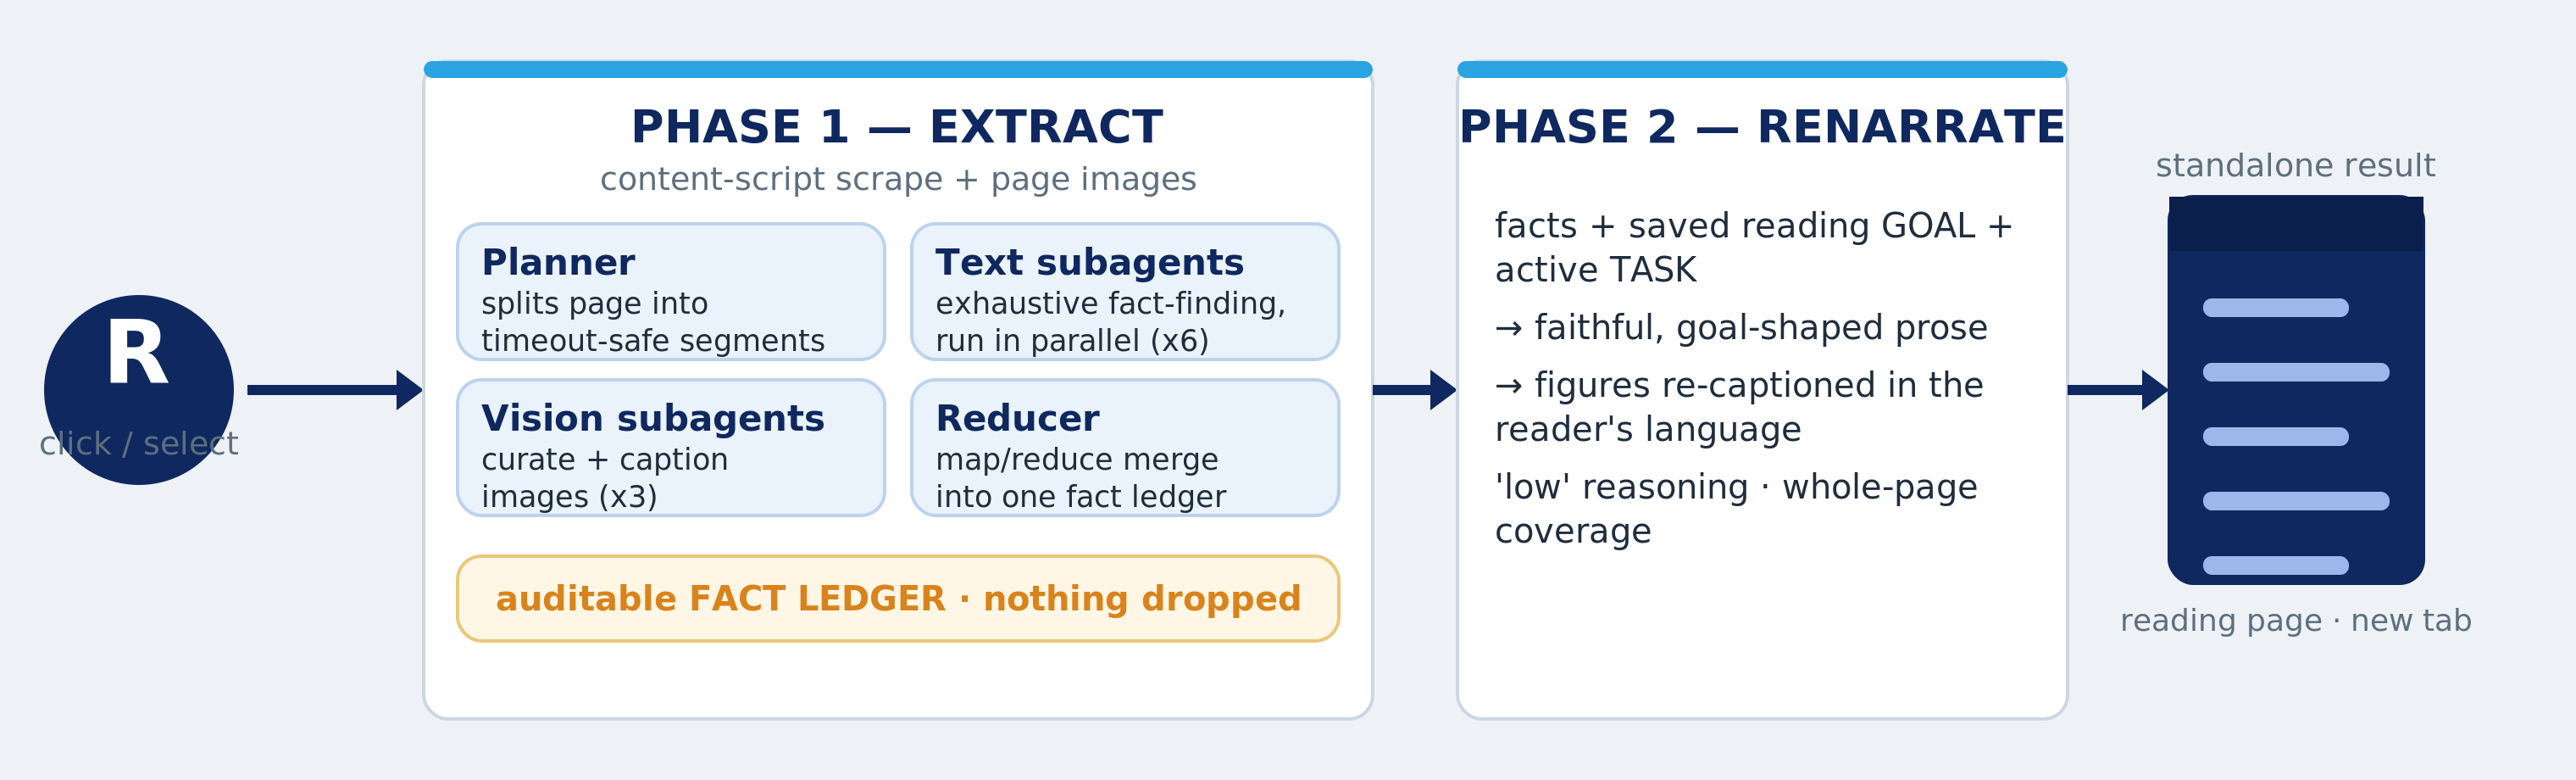
\includegraphics[width=0.82\twocolwid]{figures/fig_pipeline.png}
\caption{One click: exhaustive extraction into an auditable fact ledger, then goal-conditioned renarration into a standalone reading page.}
\end{figure}
\end{block}

\begin{alertblock}{Use Case 1 — A Parent vs.\ the Research}
A mother wants to rethink how she teaches her autistic son using new research, but the papers are a wall of jargon. Clear keeps the science exact and re-tells it through everyday analogies tied to \textit{her} goal.
\begin{figure}
\centering
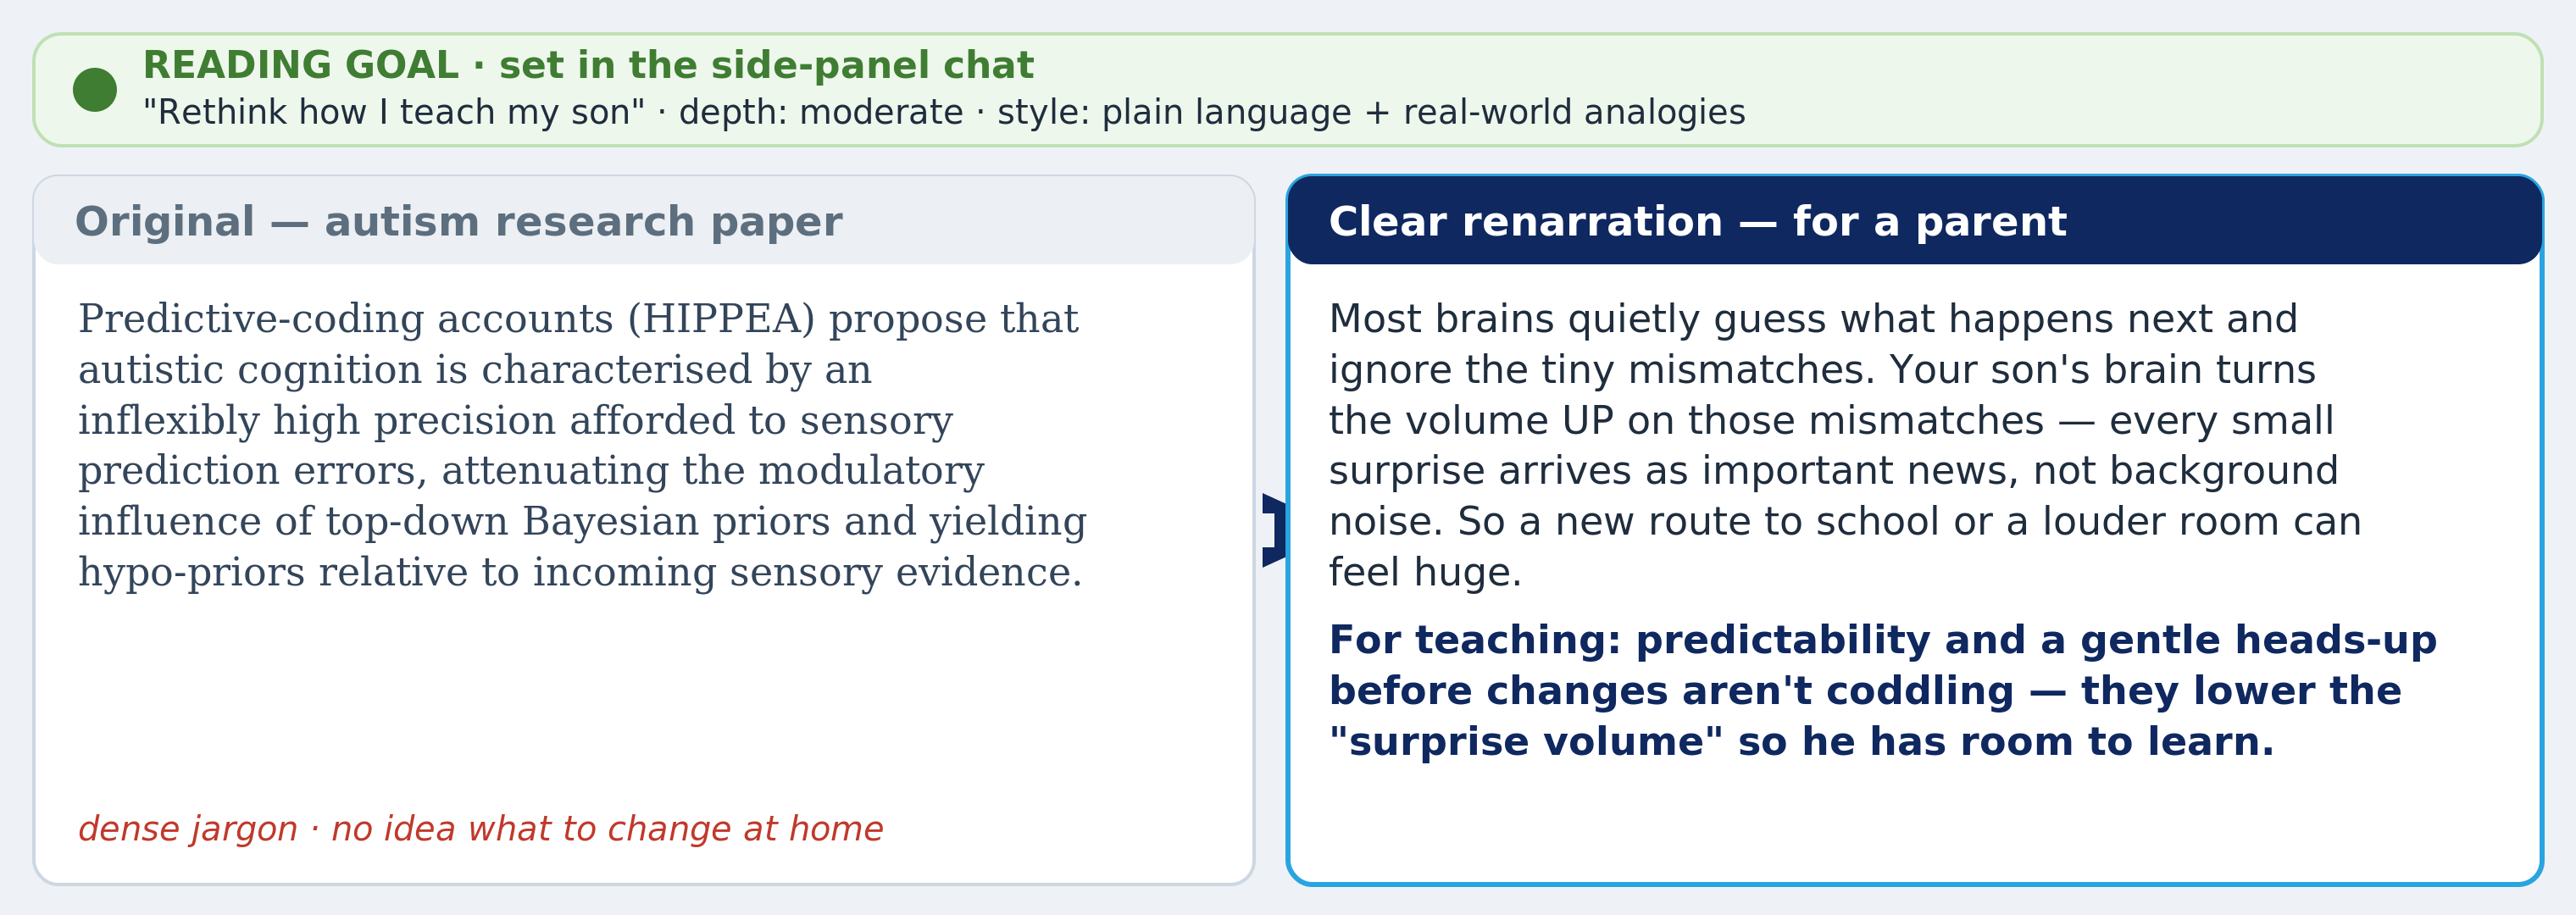
\includegraphics[width=0.80\twocolwid]{figures/fig_autism.png}
\end{figure}
\end{alertblock}

\begin{alertblock}{Use Case 2 — A Photo in Another Language That Lies}
A Spanish page shows what looks like a harmless little green apple. A non-Spanish reader would never guess it is the \textit{manchineel} — by Guinness World Records the most dangerous tree on Earth. Clear reads the foreign text and the image \textbf{together}.
\begin{figure}
\centering
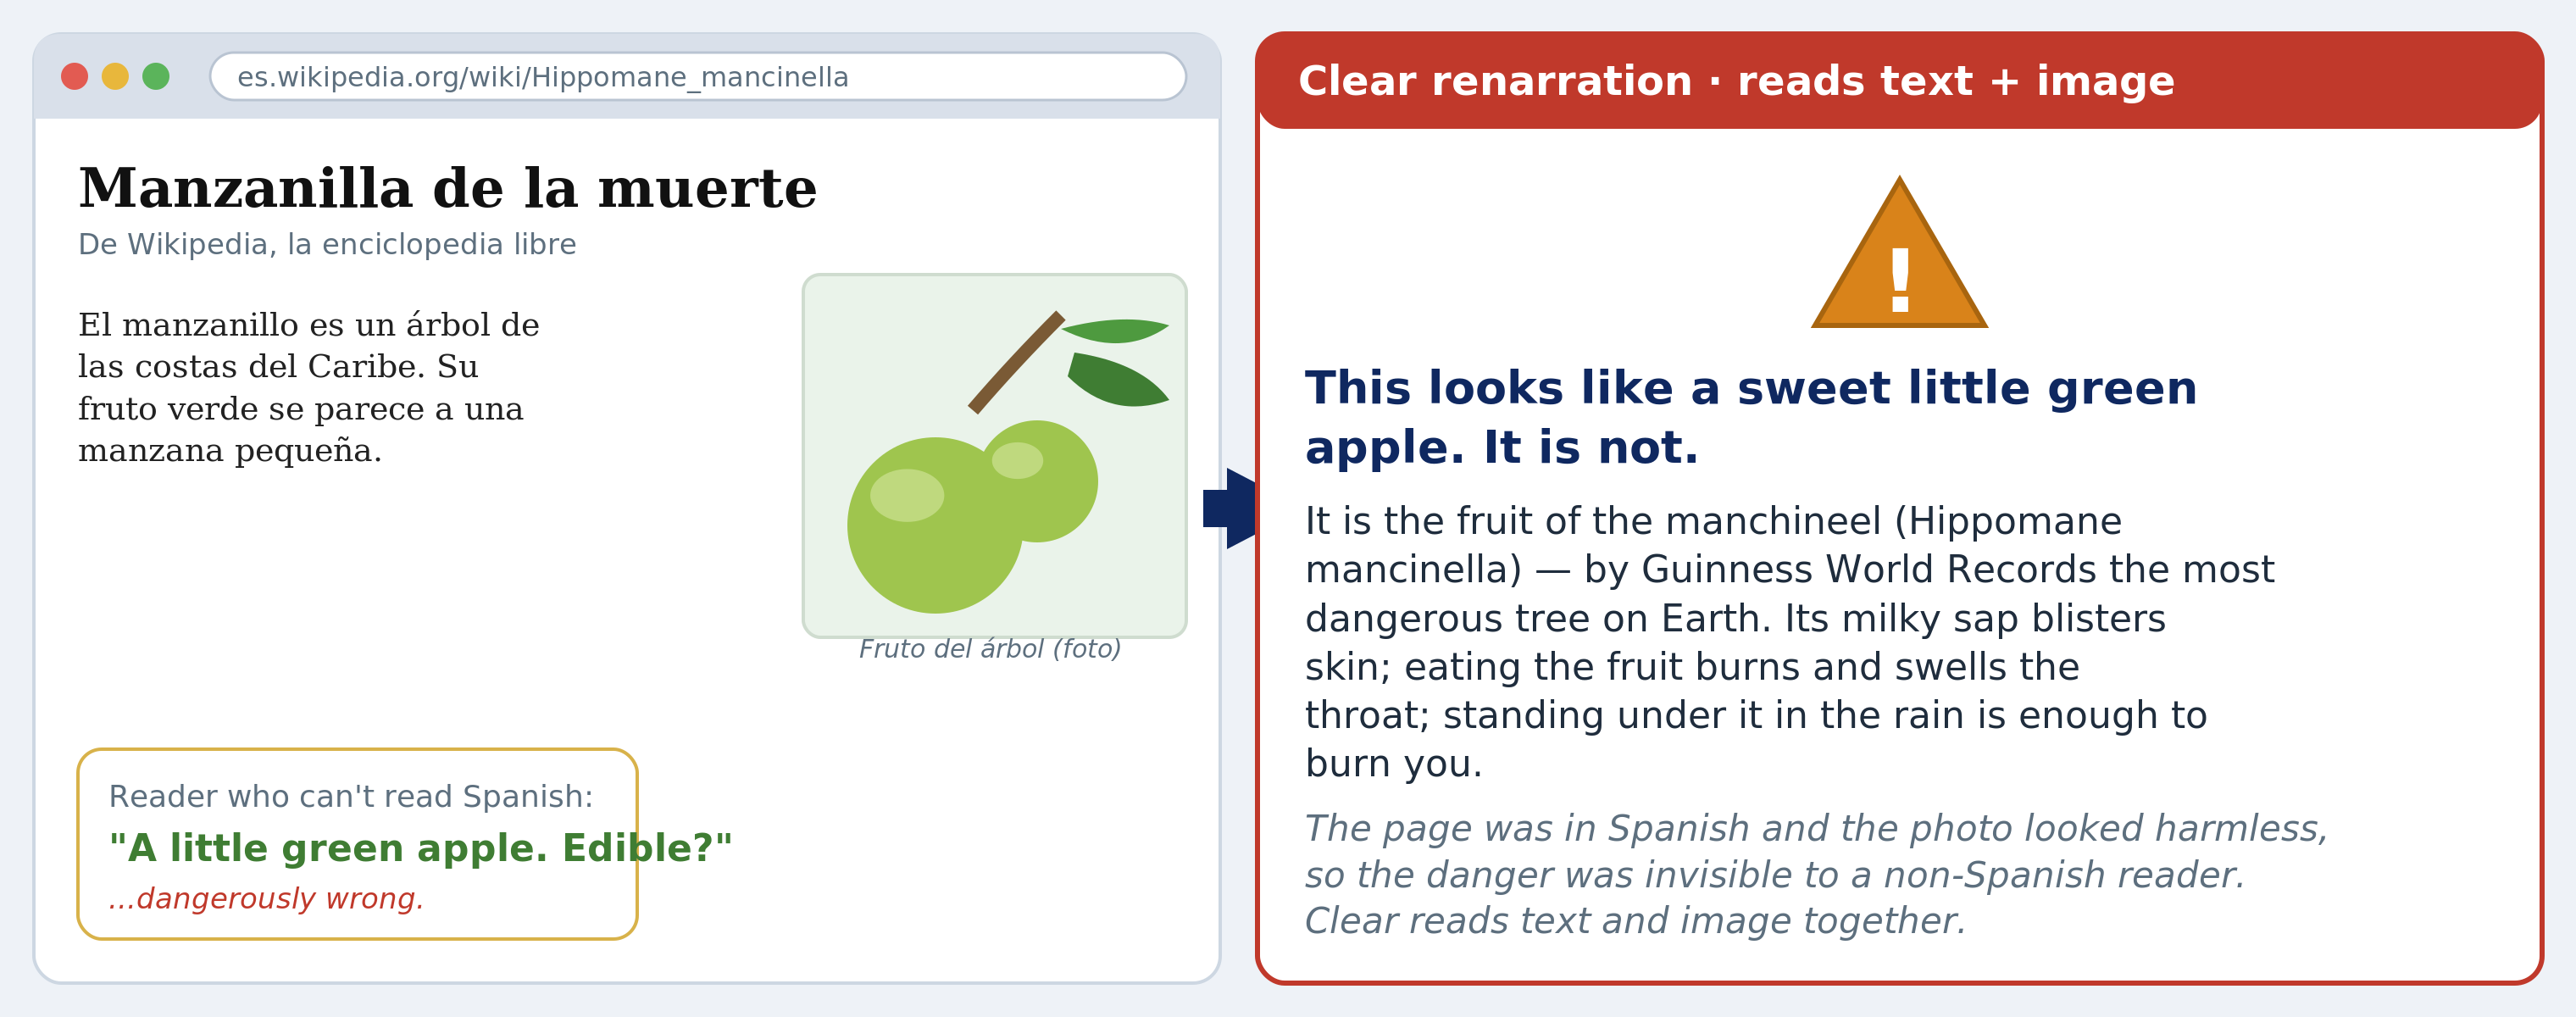
\includegraphics[width=0.74\twocolwid]{figures/fig_manchineel.png}
\end{figure}
\end{alertblock}

\end{column}

\begin{column}{\sepwid}\end{column} % spacer

%================= COLUMN 3 =================
\begin{column}{\onecolwid}

\begin{alertblock}{What Clear Buys You}
\begin{itemize}
\item \textbf{Faithful} — page-grounded; nothing invented, nothing silently dropped.
\item \textbf{Personal} — one explicit goal reshapes depth, language and analogies.
\item \textbf{Multimodal} — images are curated and explained, not discarded.
\item \textbf{Honest about coverage} — budget skips are surfaced, never hidden.
\end{itemize}
\end{alertblock}

\setbeamercolor{block alerted title}{fg=white,bg=bounblue}
\setbeamercolor{block alerted body}{fg=black,bg=white}

\begin{block}{Architecture}
\begin{itemize}
\item Chrome MV3 extension; background service worker bundled with Vite; no UI framework.
\item OpenAI Responses API wrapper — every request uses \texttt{store:\,false} (no server-side retention).
\item Budgets keep the worker under the MV3 ``unresponsive'' kill window.
\item The reading page is one self-contained HTML file with images embedded as data URIs — it works offline.
\end{itemize}
\end{block}

\begin{block}{Security Posture}
\begin{itemize}
\item A build-time API key is extractable from any shipped extension — mitigated by key rotation and budget caps; a server-side proxy / per-user key is the planned fix.
\item \texttt{<all\_urls>} is required for the on-page overlay and for embedding third-party images.
\item The overlay renders inside a \textbf{shadow DOM}; final renarrated text is written with \texttt{textContent}, never generated HTML.
\end{itemize}
\end{block}

\begin{block}{Future Work}
\begin{itemize}
\item Move credentials behind a proxy so no usable key ships in the bundle.
\item On-device / local models for fully private renarration.
\item Reader-controlled analogy depth and persistent per-domain goals.
\end{itemize}
\end{block}

\begin{block}{References}
\begin{thebibliography}{9}
\footnotesize
\bibitem{vandecruys2014} Van de Cruys, S., et al. ``Precise minds in uncertain worlds: predictive coding in autism.'' \textit{Psychological Review} 121.4 (2014): 649--675.
\bibitem{manchineel} ``Hippomane mancinella (manzanilla de la muerte).'' Wikipedia. Listed by Guinness World Records as the world's most dangerous tree.
\bibitem{openai} OpenAI. ``Responses API.'' OpenAI Platform Documentation, 2025.
\bibitem{mv3} Google. ``Chrome Extensions — Manifest V3.'' Chrome for Developers.
\end{thebibliography}
\vspace*{0.2in}
\footnotesize{\centerline{\textbf{Project}: Clear — On-Device Renarration Assistant (Chrome MV3)}}
\end{block}

\end{column}

\begin{column}{\sepwid}\end{column} % spacer
\end{columns}
\end{frame}
\end{document}
